\label{sec:evaluation}

All evaluations are performed on a quiescent Intel Core 2 dual-processor system equipped with 
16GB of RAM. 
%whereas each processor has 4 cores. 
%processor with 4 cores), with 8GB of RAM. 
Each processor is a 4-core 64-bit Intel Xeon running at 2.33 GHz with a 4MB
shared L2 cache and 32KB private L1 cache. 
The underlying operating system is unmodified CentOS 5.5, running with Linux kernel
version 2.6.18-194.17.1.el5. The glibc version is 2.5. 
In order to compare the performance fairly, all benchmarks were built as 64-bit executables 
using LLVM compiler (version 3.2). The compiler optimization level is set to ``-O1'' 
so memory allocation callsites can be reported precisely.
%since we can not report line number of source code with optimization level larger than
%``-O2''.
In our evaluation, we choose two popular benchmark suites, Phoenix~\cite{phoenix-hpca} and PARSEC~\cite{parsec}.

Our evaluations aim to answer the following questions:
\begin{itemize}
\item
  How effective is \defaults{} on detecting and predicting false sharing problem (Section ~\ref{sec:effective})?

\item
  What is the performance overhead of \defaults{} with and without prediction
  (Section ~\ref{sec:perfoverhead})?

\item
  What is the memory overhead of \defaults{}~ (Section~\ref{sec:memoverhead})?
\end{itemize}


\subsection{Detection and Prediction Effectiveness}
\label{sec:effective}

\subsubsection{Benchmarks}
To compare with state-of-the-art false sharing detection work~\cite{sheriff, OSdetection}, 
we also executes \defaults{} on two existing benchmark suites 
suites Phoenix~\cite{phoenix-hpca} and PARSEC~\cite{parsec}, 
and results are listed in the Table~\ref{table:detection}. 

%Our results show that \defaults{} not only capture previously-discovered
%false sharing, but also many detect new false sharing places. The results
%are listed in Table~\ref{table:detection}. 

%http://www.technovelty.org/tips/getting-a-tick-in-latex.html
%http://tex.stackexchange.com/questions/42619/x-mark-to-match-checkmark
%\begin{comment}
\begin{table*}[ht!]
{
\centering
\begin{tabular}{l|r|r|r}
\hline
{\bf \small Benchmark} & {\bf \small Source Code} & {\bf \small New} & {\bf \small Improvement} \\
%{\bf \small Benchmark} & {\bf \small Source Code} & {\bf \small Type of False Sharing} & {New} & {\bf \small Improvement} \\
\hline
\small \textbf{histogram} & {\small histogram-pthread.c:213} & \cmark{} & 46.22\%\\
\small \textbf{reverse\_index} & {\small reverseindex-pthread.c:511} & \xmark{} & 0.09\%\\
\small \textbf{word\_count} & {\small word\_count-pthread.c:136} & \xmark{} & 0.14\%\\
\hline
\small \textbf{streamcluster} & {\small streamcluster.cpp:985} & \xmark{} & 7.52\% \\
\small \textbf{streamcluster} & {\small streamcluster.cpp:1907} & \cmark{} & 4.77\%\\
%\small \textbf{bodytrack} & {\small TrackingModel.cpp:59} & 0 & \cmark{} & \\
\hline
\hline
\small \textbf{linear\_regression} & {\small linear\_regression-pthread.c:133} & \xmark{} & 1206.93\%\\
\hline
\end{tabular}
\caption{Detection results of \defaults{} on Phoenix and PARSEC benchmark suites. \label{table:detection}}
}
\end{table*}

In this table, the first column lists those programs with false sharing problems. 
The second column shows precisely where the problem is. Actually, all false sharing found
are internal object false sharing on heap objects, although \defaults{} has no 
problem to find intern-objects and global false sharing. So the memory allocation site 
are listed in the table.
The third column ``New'' marks whether this false sharing is newly found by \defaults{} or not.
False sharing found by previous work are marked as cross mark(\xmark{}) and those 
newly found false sharing are identified using a tick mark(\cmark{}). 
The last column ``Improvement'' shows the performance improvement after fixing false sharing 
based on the average result with $10$ runs. 
The improvement rate is calculated by substracting $1$ from normalized runtime. Taking 
\texttt{histogram} for an example here, original runtime of \texttt{histogram} is $0.75s$
and new runtime is $0.51s$, then the performance improvement is $(0.75/0.51) - 1$.

Seen from the table, \defaults{} reveals several unknown false sharing problems. \defaults{} detects 
false sharing in \texttt{histogram} and additional false sharing in line 1908 of
\texttt{streamcluster}. 
In \texttt{histogram}, multiple threads repeatedly modify different locations of the same heap object. 
Padding the data structure \texttt{thread\_arg\_t} fixes the false sharing problem and 
helps to improve the performance around 46\%.
In \texttt{streamcluster}, multiple threads are changing a \texttt{bool} array, \texttt{switch\_membership}, simultaneously. By simply changing this array to \texttt{long} type contributes to about 4.7\% performance improvement. 
%None of these two false sharing problems has been reported by previous tools.

Other false sharing problems has been revealed by previous tool \sheriff{}~\cite{sheriff}. 
Same as \sheriff{}, we didn't see much performance improvement for \texttt{reverse\_index} and 
\texttt{word\_count} since number of updates inside them is not a significant number. But they
are actually false sharing problems that have been verified manually by us.

\texttt{streamcluster} has another false sharing problem that different threads 
may change the same object simultaneously. 
Actually authors of \texttt{streamclsuter} have already realized possible
false shairing problems and meant to utilize a macro \texttt{CACHE\_LINE} to avoid it. Unfortunately,
the defaulted value of this macro is setted to $32$ bytes, which is different with the actual
cache line size that we are using. By setting to $64$ bytes instead, we see around $7.5\%$ performance
improvement.

linear\_regression has a significant false sharing problem. 
Different threads simultaneously changed an array of thread-indexed structures in a tight
loop, which causes a huge amount of cache invalidations. 
Fixing false sharing inside can improve the performance for $12\times$. 
Actually, if we do not enable prediction then 
we can not detect false sharing problem inside because false sharing behavior is 
very sensitive to the starting address of false sharing object. 
We are going to explore this more detailed in Section~\ref{sec:predicteval}.
Since \defaults{} are using a customized memory manager, which may
bring us different allocation metadata and different memory map for allocation,
false sharing problem may not manifest with ``-O1'' optmization flag of \texttt{clang}.
%http://tex.stackexchange.com/questions/42619/x-mark-to-match-checkmark
%\begin{comment}

\subsubsection{Real Applications}
To verify its practicability, we further evaluate \defaults{} 
on several widely-used real applications, which none of previous work has considered.  
These real applications include a server application \texttt{MySQL}~\cite{mysql}, 
a common C++ library \texttt{boost}~\cite{libfalsesharing} 
and a distributed memory object caching system \texttt{memcached}, a network retriver \texttt{aget}, 
a parallel bzip2 file compressor \texttt{pbzip2} and a parallel file scanner \texttt{pfscan}.
Among them, \texttt{MySQL} and \texttt{boost} are known to have some false sharing problem inside 
so we evaluate their specific versions, \texttt{MySQL-5.5.32} and
\texttt{boost-1.49.0}.

False sharing in \texttt{MySQL} has caused significant scalability problem and
it was very difficult to be identified. 
According to the architect of \texttt{MySQL} Mikael Ronstrom, ``we had gathered specialists on 
InnoDB..., participants from MySQL support... and a number of generic specialists on 
computer performance...'', ''the fruit of the meeting ... were able to 
improve \texttt{MySQL} performance by 6$\times$ with those scalability fixes''. 
The false sharing of boost library is caused by the special usage of \texttt{spinlock} pool and fixing
it brings 40\% performance improvement. 
\defaults{} is able to succesfully detect false sharing locations
in \texttt{MySQL} and \texttt{boost} library. 
For the other four applications, \defaults{} doest not find serere false sharing problems.

\subsubsection{Prediction Effectiveness}
\label{sec:predicteval}
We evaluates the prediction effectiveness of \defaults{} on the \texttt{linear\_regression} benchmark.
We choose this benchmark for two reasons:
\begin{enumerate}
\item
False sharing problem of this benchmark can not be detected without prediction. 

\item
This benchmark has a severe performance problem when false sharing actually occurs, which should be 
detected but can be omitted by exiting tools.
\end{enumerate}

The data structure of false sharing object and the source code
to experience false sharing is showed in Figure~\ref{fig:linearregression}. 
When we are using \texttt{clang} compiler while compiling for $64$bit binary, the size of this 
data structure is $64$ bytes.

\begin{figure}[!h]
{\centering
\subfigure{\lstinputlisting[numbers=none,frame=none,boxpos=t]{fig/linearregression.psedocode}}
%\hspace{30pt} 
%\subfigure[False sharing with different alignment]{%
%   \label{fig:lr_perf}
%   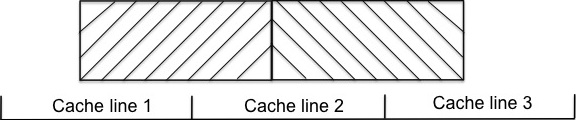
\includegraphics[width=0.36\textwidth]{fig/Potential3.jpg}}
\caption{False sharing problem inside \texttt{linear\_regression} benchmark.
\label{fig:linearregression}}
}
\end{figure}

\begin{figure}[!h]
\begin{center}
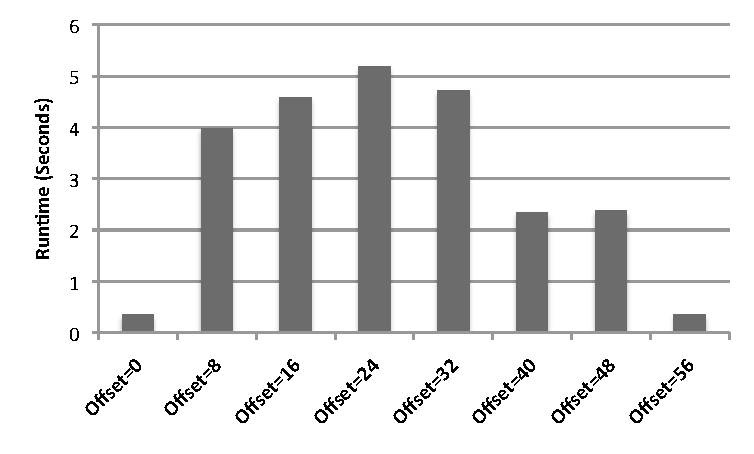
\includegraphics[width=3.3in]{fig/perfsensitive}
\end{center}
\caption{
Inside \texttt{linear\_regression} benchmark,
performance is sensitive to the offset between starting address of the false sharing object 
and the starting of cache line 
\label{fig:perfsensitive}}
\end{figure}

For this false sharing problem, the main thread allocates an array of $8$ elements 
(if $8$ cores totally), 
with each element being a \texttt{lreg\_args} type. 
Then this array will be passed to different threads so that they can only updates its 
thread-dependent area, see Figure~\ref{fig:linearregression}.
Actually, different fields of this data structure \texttt{lreg\_args} has different access pattern:
only those fields between $SX$ and $SXY$ (totally around $40$ bytes) are constantly read and updated.

Thus, \texttt{linear\_regression} actually is very sensitive to the starting address 
of the false sharing object, which can be caused by many of dynamic properties 
listed in Section~\ref{sec:intro}, e.g.,
hardware platform, optimization flag, compiler etc.
This sensitivity can be seen in Figure~\ref{fig:perfsensitive}.
That is, when offset is $0$ or $56$ bytes, there is no false sharing at all.
Actually, using our customized memory manager,
the offset between the starting address of potential false sharing object 
and starting of cache line is actually $56$ bytes,
that explain why we can not detect false sharing problem without prediction enabled.

\defaults{} can predict false sharing problem precisely for all of these cases. This explains
the effectiveness of prediction tool.

\subsection{Performance Overhead}
\label{sec:perfoverhead}
To avoid the effect caused by extreme outliers,
all performance data are based on the average of 10 runs excluding the
maximum and minimum values.
Actual performance overhead can be seen in the following figure~\ref{}. 


\subsection{Memory Overhead}
\label{sec:memoverhead}
Since \defaults{} pre-allocates a huge block of memory using \texttt{mmap} system call for 
its heap usage, 
virtual memory can not be used to tell actual memory overhead imposed by our tool. 
Hence, we only evaluate the physical memory overhead used by an application only. 
This number is based on proportional set size (PSS) in \texttt{/proc/self/smaps}
as discussed by Justin et al. ~\cite{memusage}. 

When evaluating an application, we start a script program to save 
corresponding \texttt{smaps} files periodically. 
The maximum number of total physical memory usage is selected for calculation.
%It is noted that we remove the physical memory usage of   
Results of memory usage is shown in Figure~\ref{fig:memusage}. As we can see,
\defaults{} does not increase memory usage substantially in all cases except for \texttt{swaptions}. 
Specifically, removing \texttt{swaptions} from calculation reduces 
the average memory overhead from 64\% to 22\%. 

The reason of \texttt{swaptions} using a large amount of memory is that 
its original memory usage is too small (only 3KB), and 
the additional memory added by \defaults{} in detection, prediction and
reporting yields a large number in percentage calculation. 

\begin{figure*}
\begin{center} 
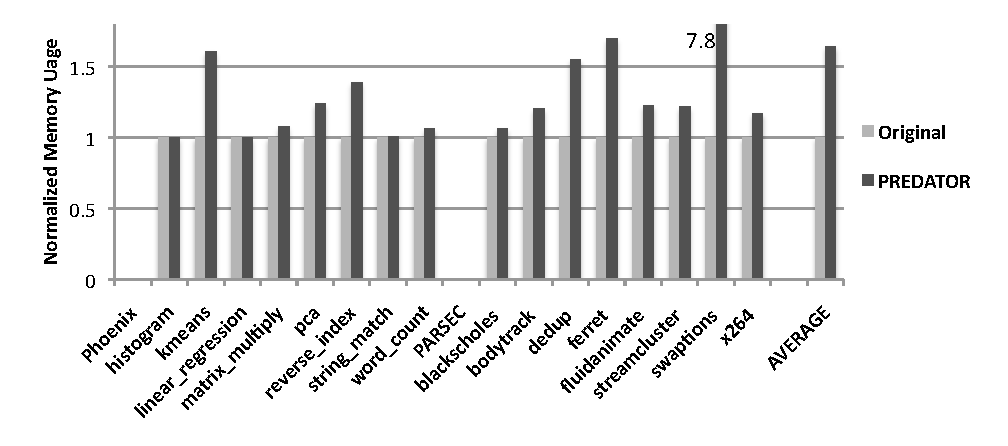
\includegraphics[width=5in]{fig/memusage}
\end{center}
%\includegraphics{fig/potential.pdf}
\caption{Memory usage overhead}
\label{fig:memusage}
\end{figure*}


